%% Results chapter
%% author Liu Peng

After designing, implementing and testing the application. We started several evaluation tests on the streaming performance. Finally we had released the application in Google Play Store in Nov 2013. So far, we have improved the application in many aspects and also brought many new features to it. During the past one year, we have accumulated many useful data and interesting results. In this chapter we will present and analyze those results.

\subsection{Performance}
In terms of streaming, our solution include two major streaming components. It would be helpful to study and compare which streaming protocol have the better performance while streaming multimedia contents. Moreover, by comparing different streaming types of media, we could investigate which protocol is best suitable for certain type of media. \\
\\Two major streaming technology we used in our solution are HTTP streaming and RTSP streaming.\\
\\
Hypertext Transfer Protocol (HTTP) refers to the protocol used to deliver web pages and images across the Internet worldwide. HTTP is an adopted, open standard and the most ubiquitous mode of delivery on-line. HTTP can be delivered by a variety of web servers, both commercial and open source.\\
\\
Real Time Streaming Protocol (RTSP) is a network control protocol used in entertainment and communications systems to control streaming media servers. RTSP is used to establish and control media sessions between two points, usually server and player client. Clients of media servers issue VCR-like commands, such as PLAY and PAUSE, to facilitate real-time control of playback of media files from the server. AirPlay uses RAOP, a RTSP-like streaming protocol, for the streaming of iTunes music. \\
\\
Since we have both protocols implemented in our application. We could compare the performance by streaming the same content to two receivers using different protocol. We selected a mp3 music file and try to stream it to an AirPlay Speaker and an DLNA Speaker, and we used Wireshark running on rooted Android phone to capture the packets in the network.\\
\\
The result is presented below, the initial packet count is relatively high. This is because there is a lot multicast messages in the network for device discovery. After that, streaming graph shows that after an initial increase in the traffic, network traffic enters a relatively stable state. This is because the TCP protocol reaches the best optimized transmission speed.\\
\\
Next, we added packet loss in the network and compare the influence to the two streaming process. The result is shown in Figure below:
\begin{figure}[H]
\begin{minipage}[b]{0.45\linewidth}
\centering
\includegraphics[width=\textwidth]{charts/AirPlay_traffic_data}
%%\hspace{0.1cm}
\end{minipage}
\begin{minipage}[b]{0.45\linewidth}
\centering
\includegraphics[width=\textwidth]{charts/AirPlay_traffic_5loss_data}
\end{minipage}
\begin{minipage}[b]{0.45\linewidth}
\centering
\includegraphics[width=\textwidth]{charts/AirPlay_traffic_10loss_data}
%%\hspace{0.1cm}
\end{minipage}
\begin{minipage}[b]{0.45\linewidth}
\centering
\includegraphics[width=\textwidth]{charts/AirPlay_traffic_15loss_data}
\end{minipage}
\caption{AirPlay streaming performance in terms of packet loss}\label{multiavp}
\end{figure}



\begin{figure}[H]
\begin{minipage}[b]{0.45\linewidth}
\centering
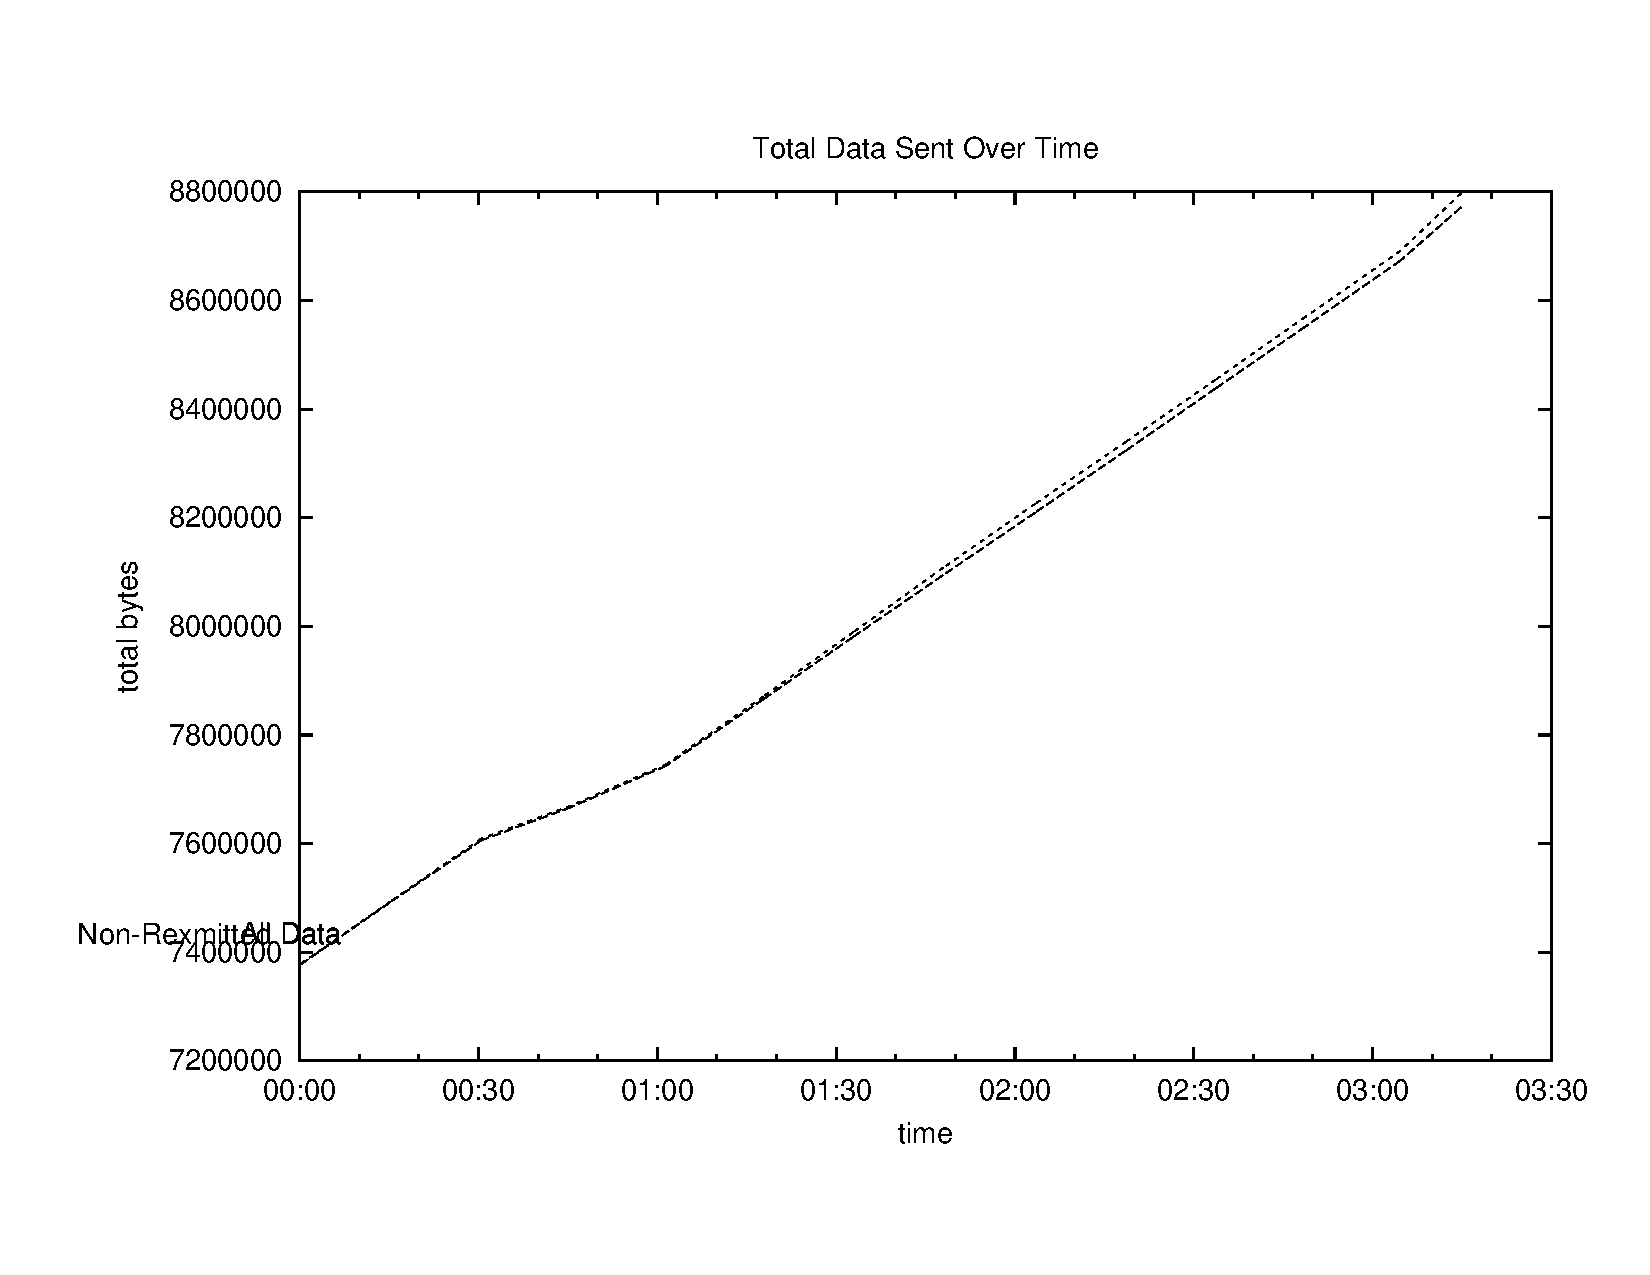
\includegraphics[width=\textwidth]{charts/dlna_traffic_data}
%%\hspace{0.1cm}
\end{minipage}
\begin{minipage}[b]{0.45\linewidth}
\centering
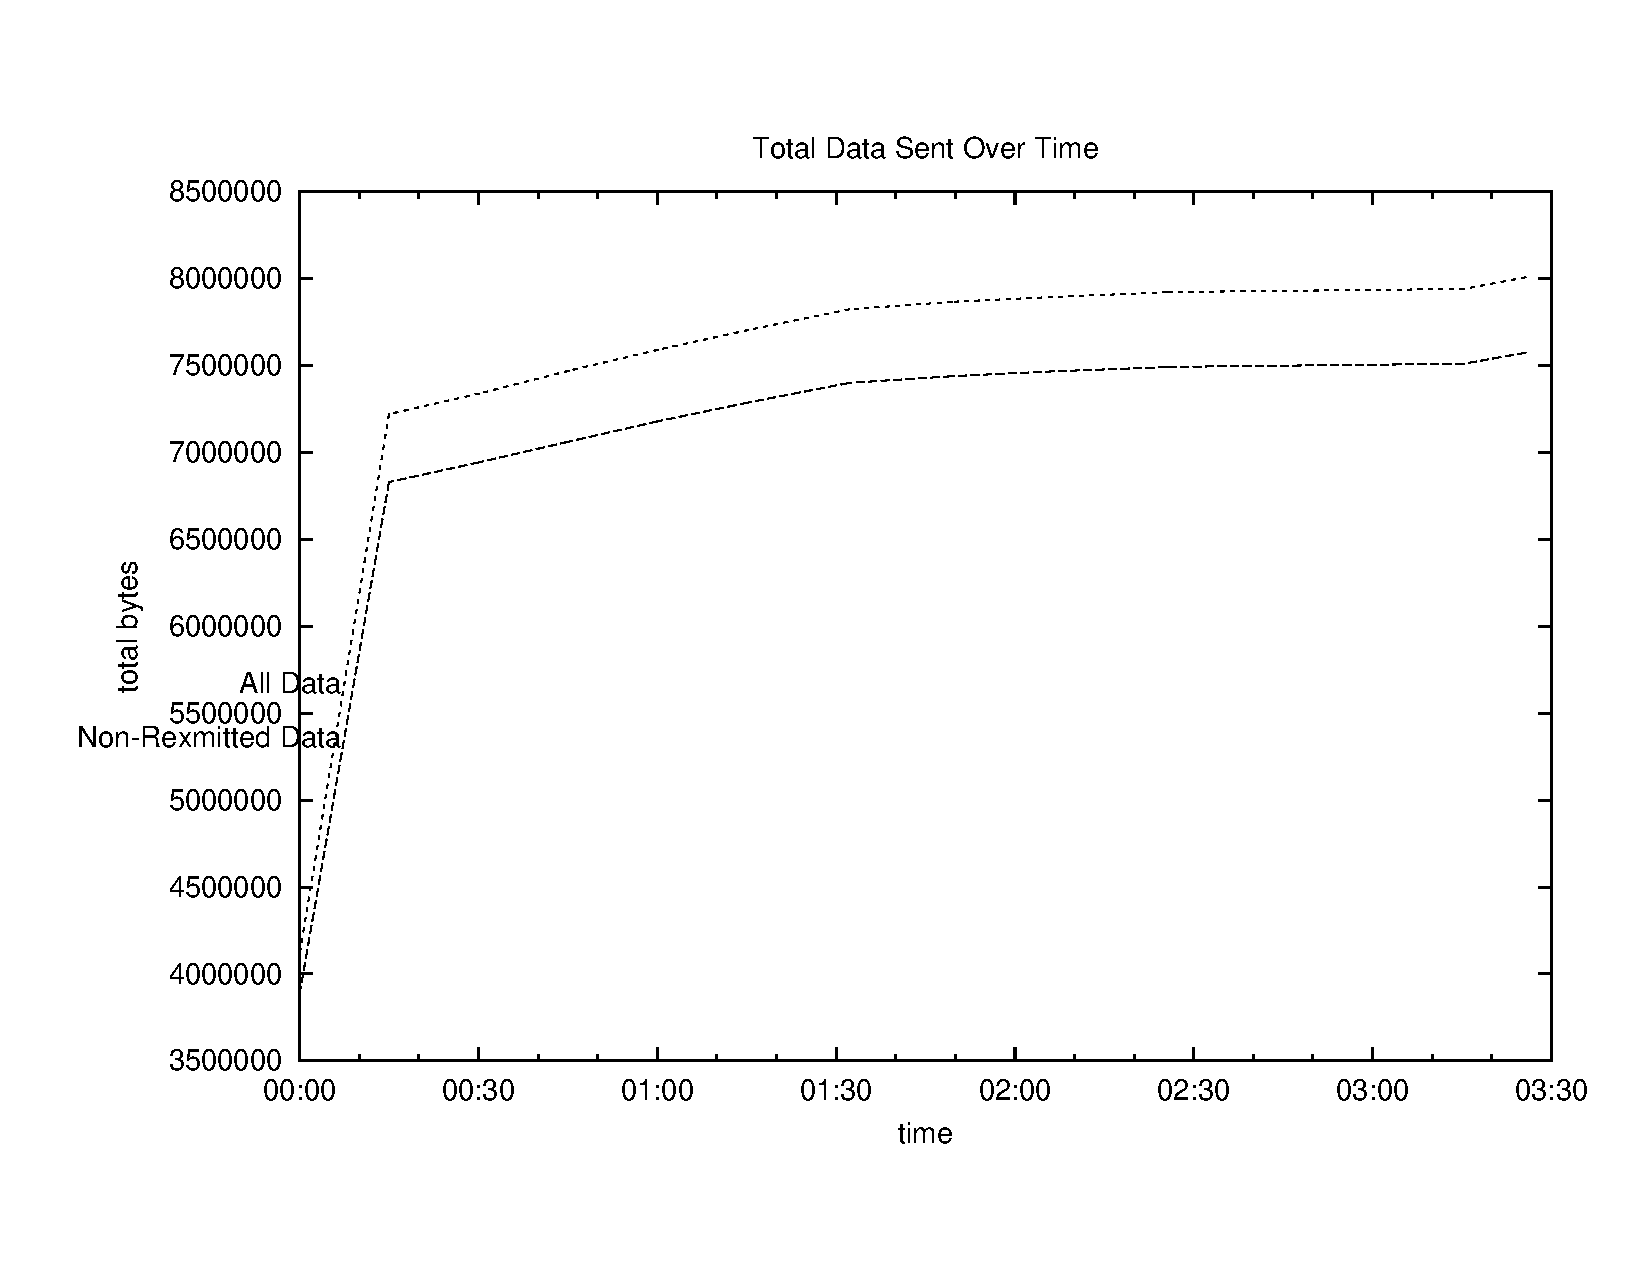
\includegraphics[width=\textwidth]{charts/dlna_traffic_5loss_data}
\end{minipage}
\begin{minipage}[b]{0.45\linewidth}
\centering
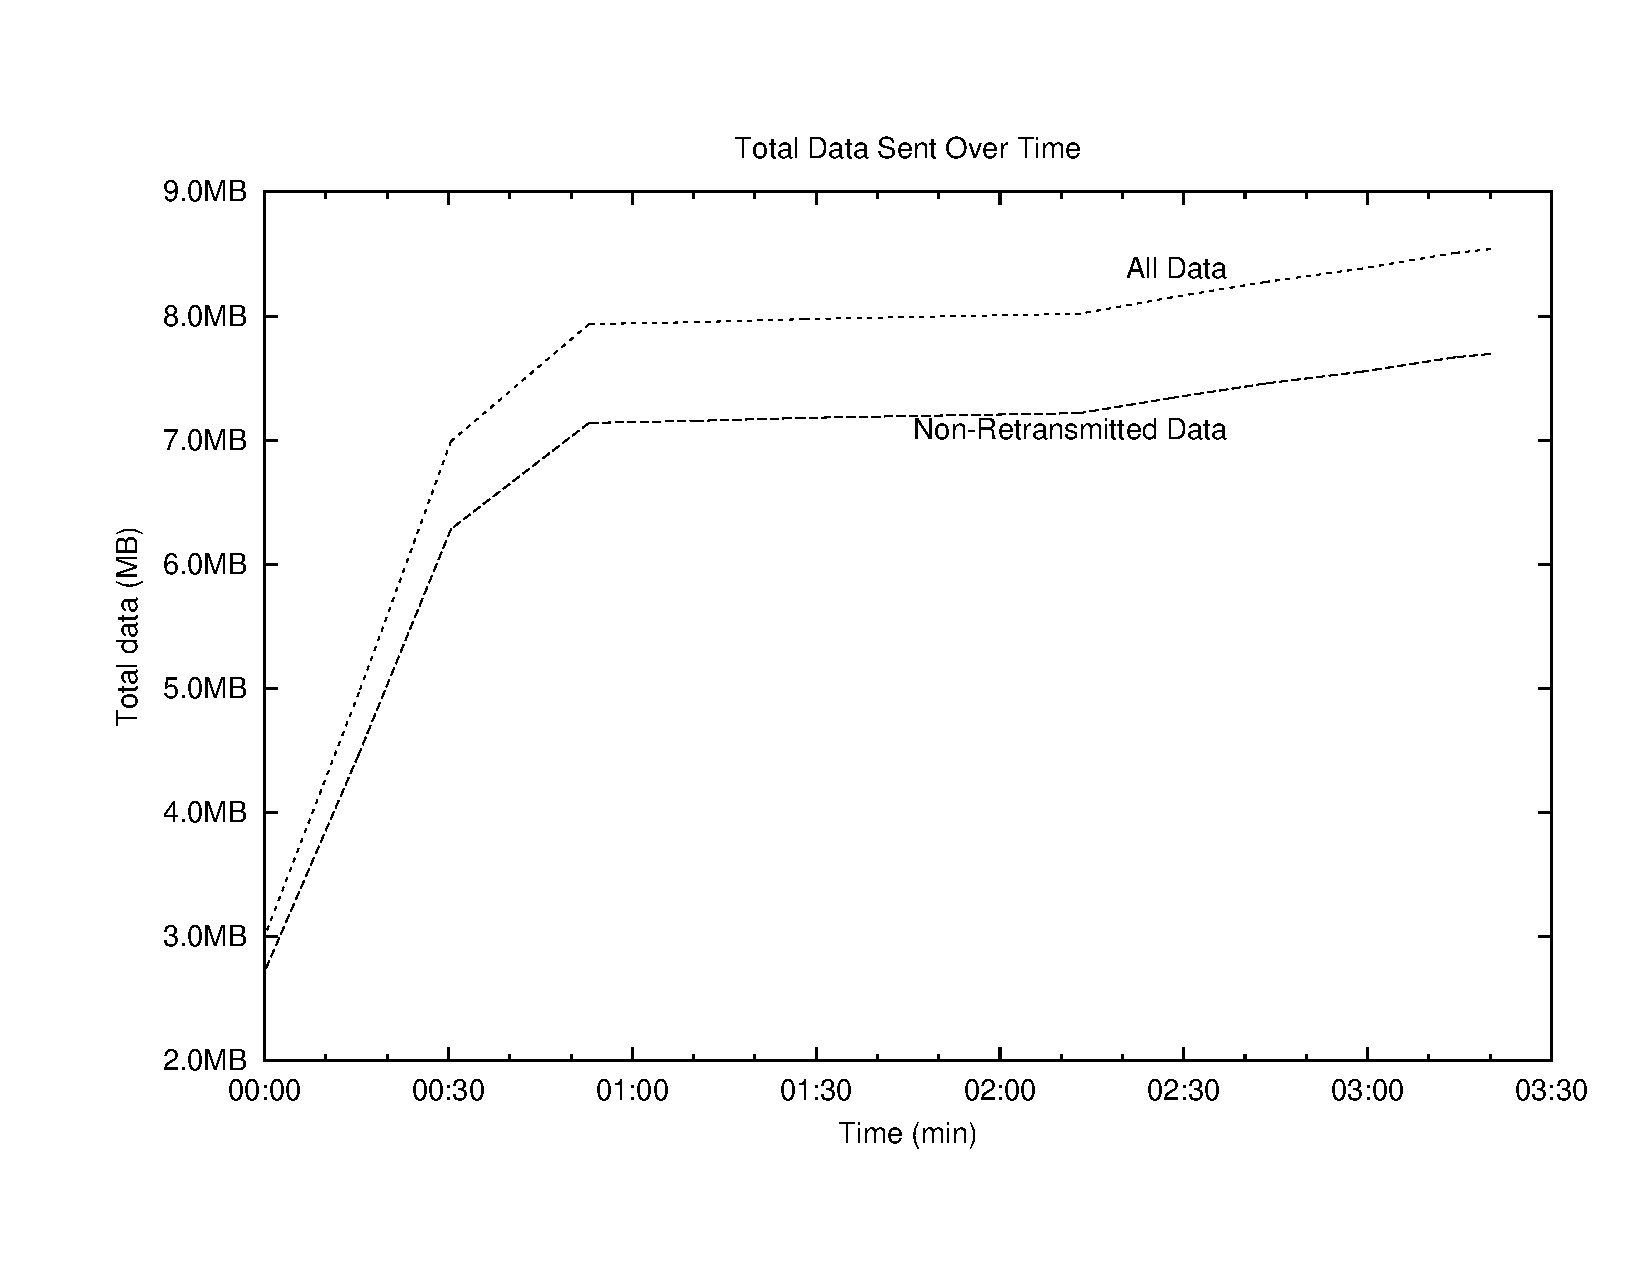
\includegraphics[width=\textwidth]{charts/dlna_traffic_10loss_data}
%%\hspace{0.1cm}
\end{minipage}
\begin{minipage}[b]{0.45\linewidth}
\centering
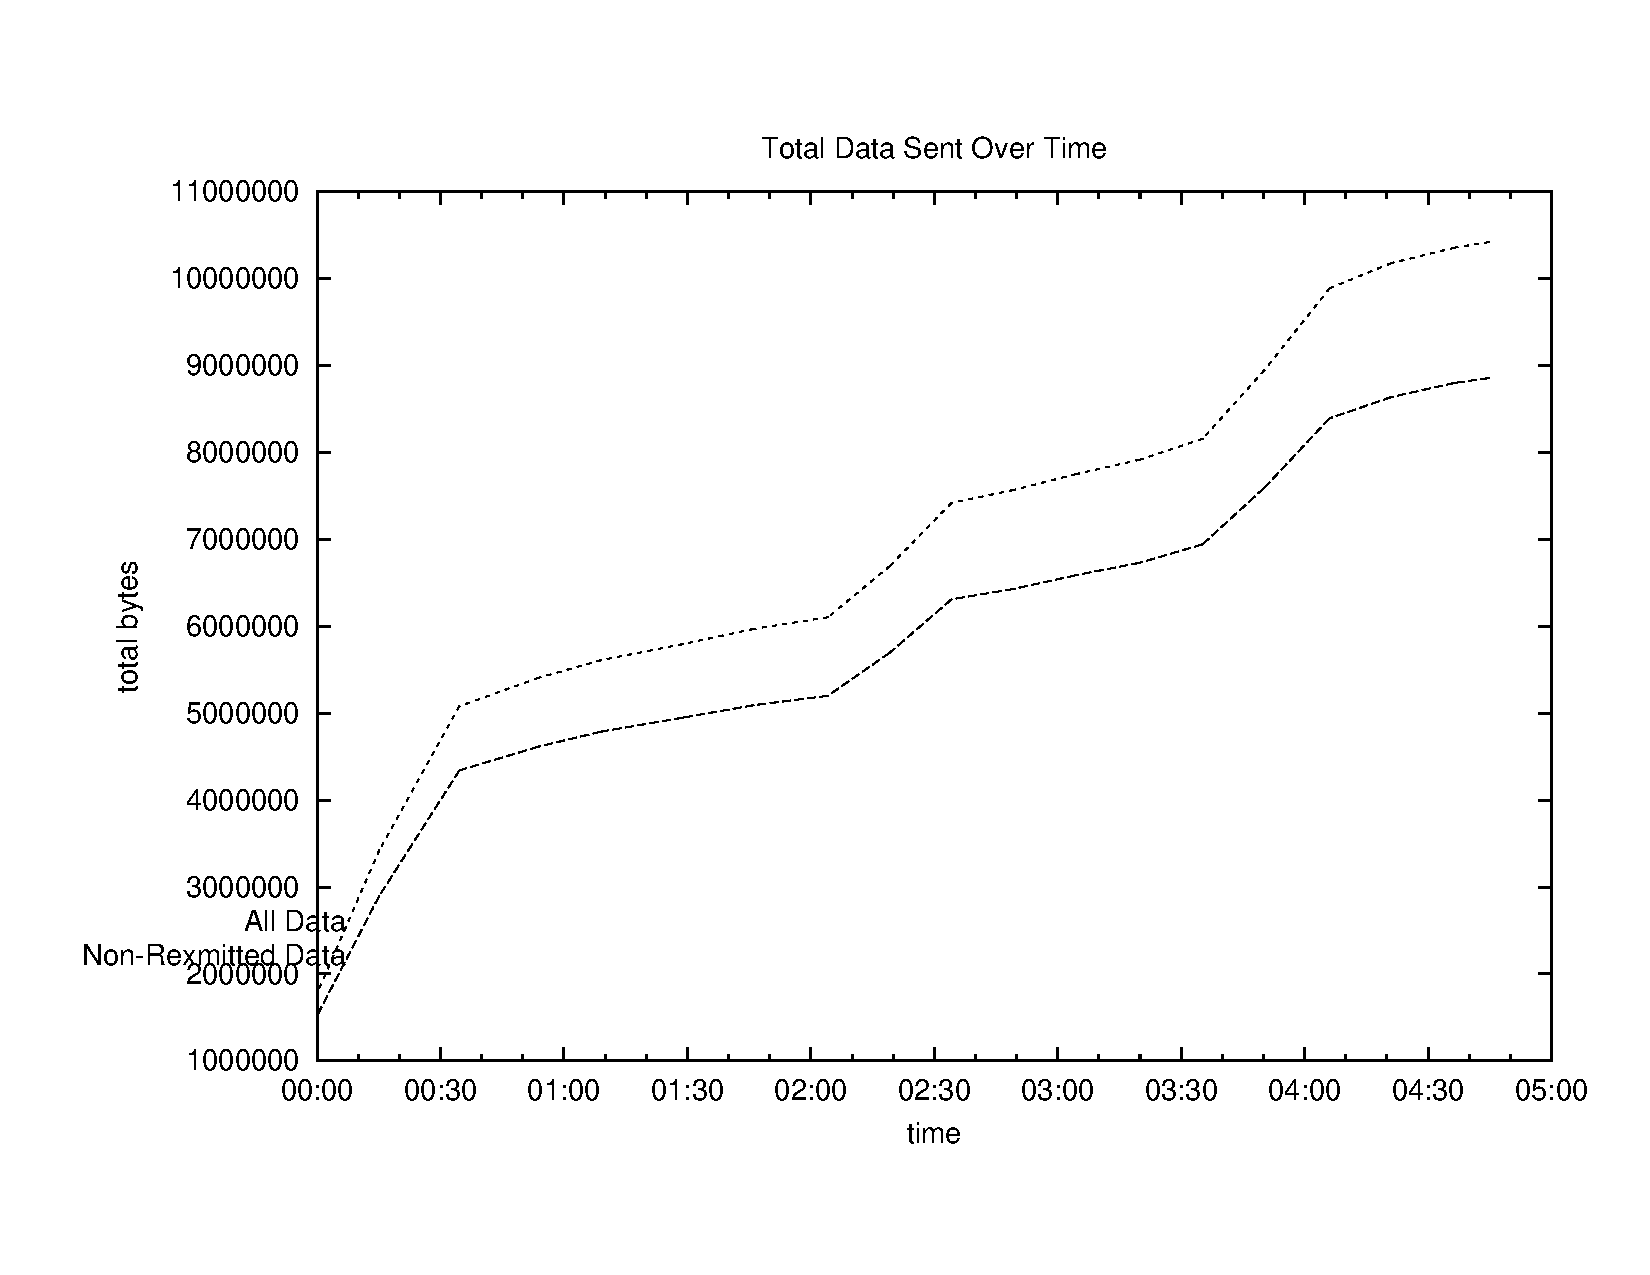
\includegraphics[width=\textwidth]{charts/dlna_traffic_15loss_data}
\end{minipage}
\caption{DLNA streaming performance in terms of packet loss}\label{multiavp}
\end{figure}

\begin{figure}[htb]
\centering \includegraphics[height=10cm]{charts/AirPlay_traffic_data}
\caption{AirPlay traffic data chart \label{chart6}}
\end{figure}
\begin{figure}[htb]
\centering 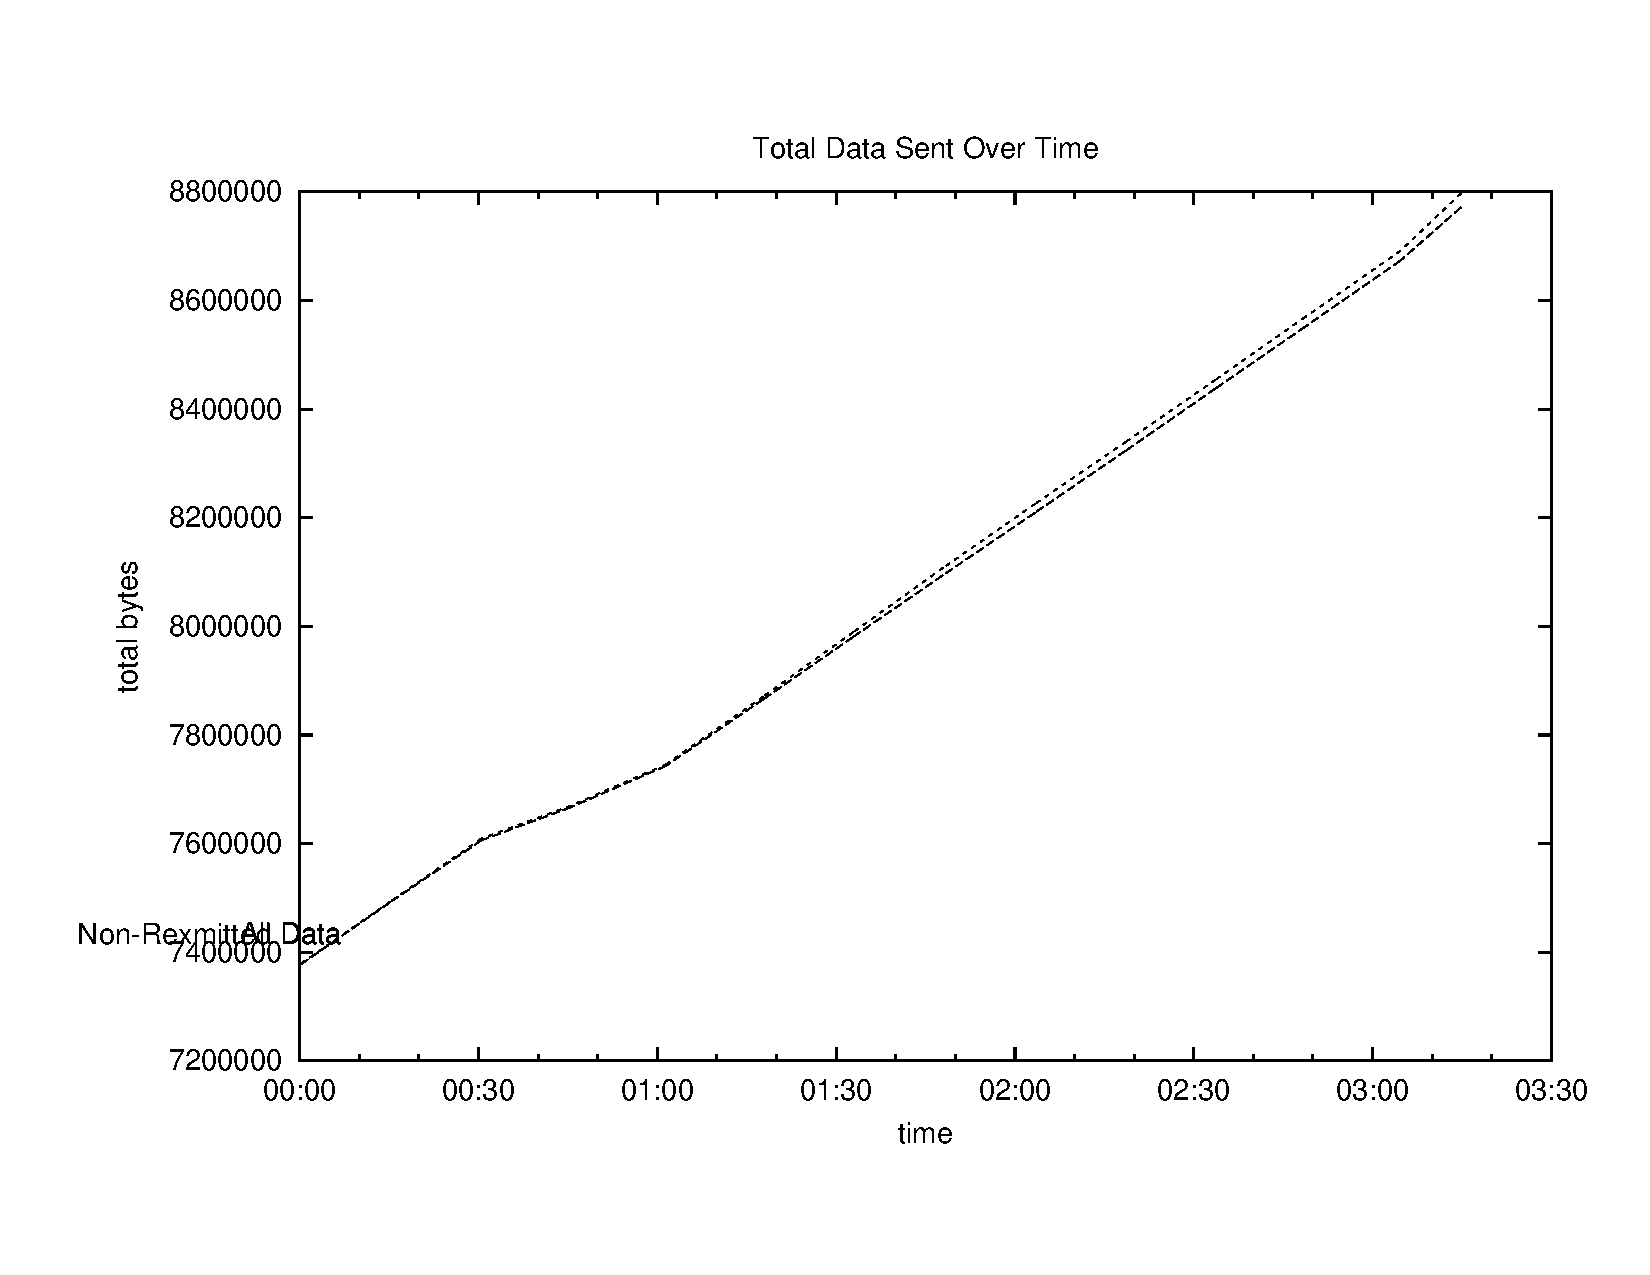
\includegraphics[height=10cm]{charts/dlna_traffic_data}
\caption{DLNA traffic data chart \label{chart6}}
\end{figure}

\begin{figure}[htb]
\centering \includegraphics[height=10cm]{charts/badnetwork_AirPlay_traffic_data}
\caption{AirPlay bad network traffic data chart \label{chart6}}
\end{figure}
\begin{figure}[htb]
\centering 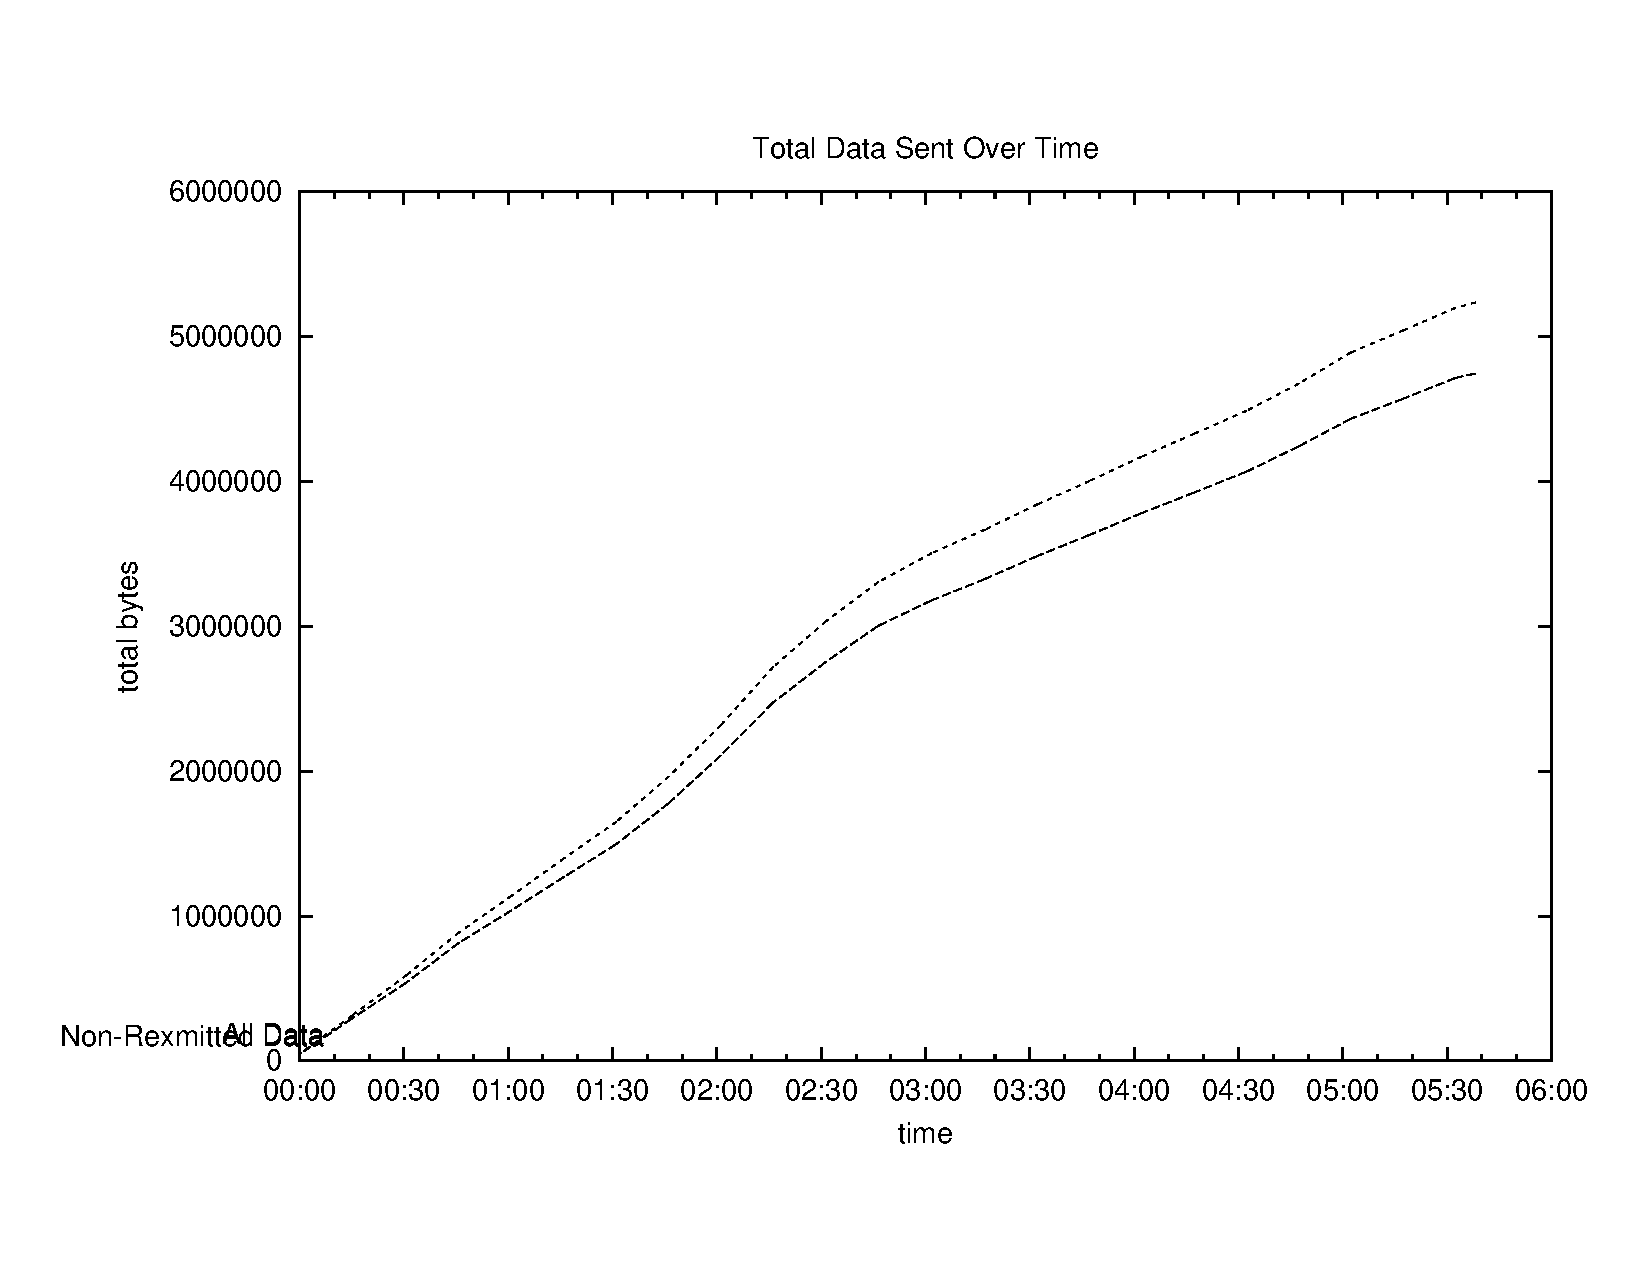
\includegraphics[height=10cm]{charts/badnetwork_dlna_traffic_data}
\caption{DLNA bad network traffic data chart \label{chart6}}
\end{figure}


\begin{figure}[htb]
\centering \includegraphics[height=10cm]{charts/AirPlay_traffic_5loss_data}
\caption{AirPlay bad network traffic data chart \label{chart6}}
\end{figure}
\begin{figure}[htb]
\centering 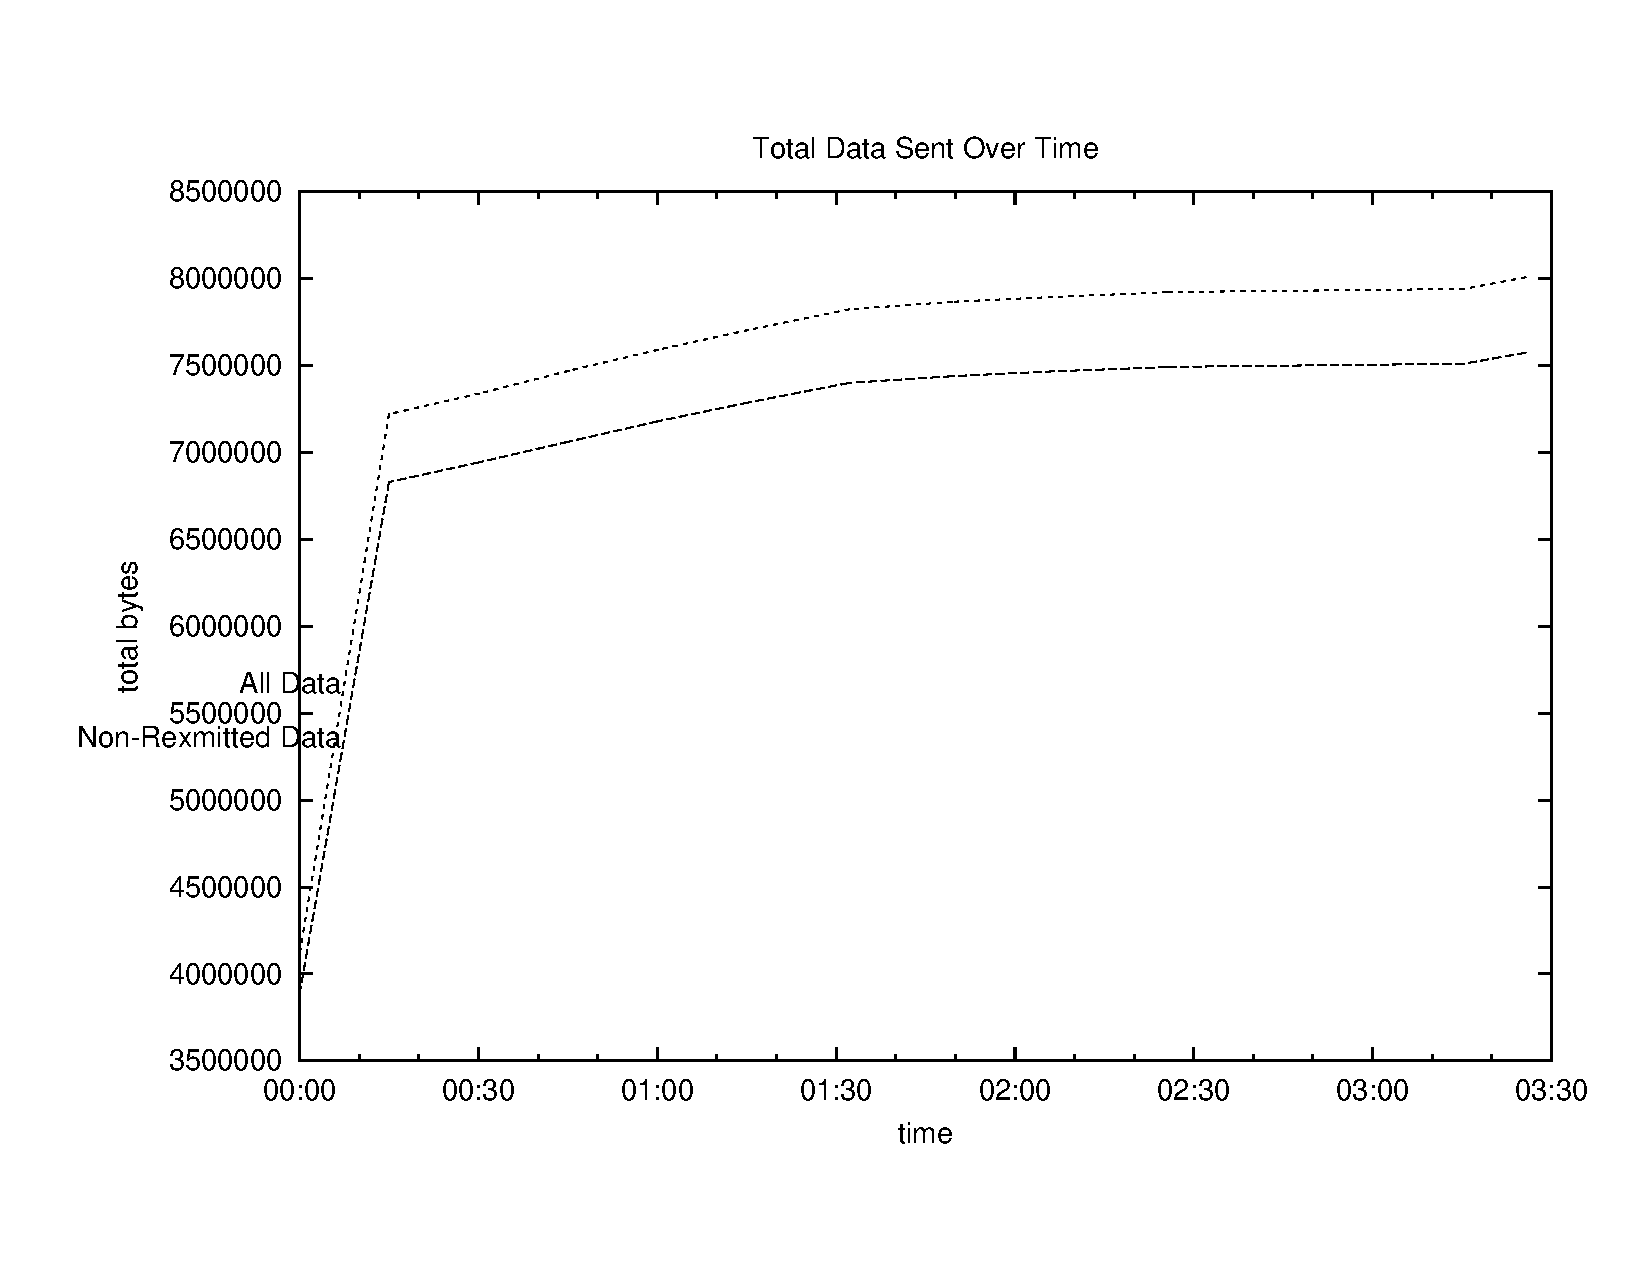
\includegraphics[height=10cm]{charts/dlna_traffic_5loss_data}
\caption{DLNA bad network traffic data chart \label{chart6}}
\end{figure}


\begin{figure}[htb]
\centering \includegraphics[height=10cm]{charts/AirPlay_traffic_10loss_data}
\caption{AirPlay bad network traffic data chart \label{chart6}}
\end{figure}
\begin{figure}[htb]
\centering 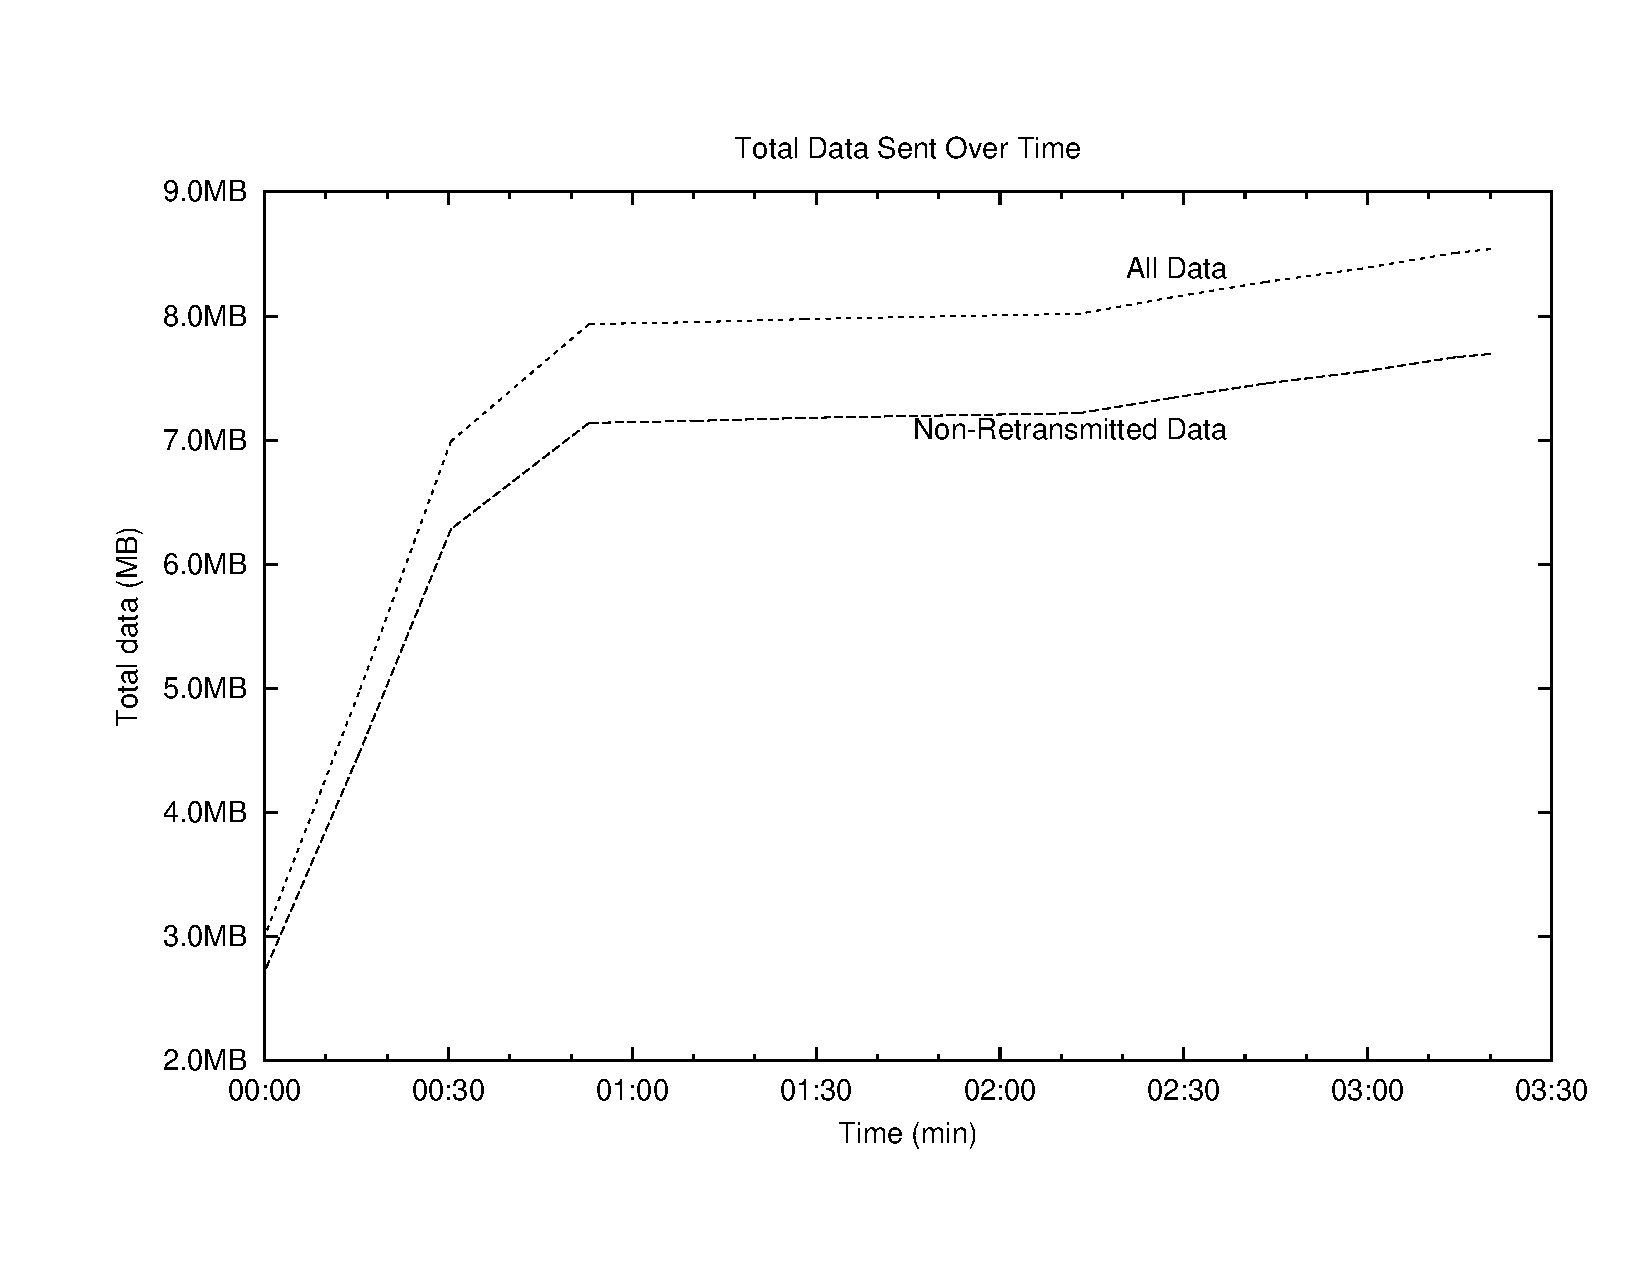
\includegraphics[height=10cm]{charts/dlna_traffic_10loss_data}
\caption{DLNA bad network traffic data chart \label{chart6}}
\end{figure}


\begin{figure}[htb]
\centering \includegraphics[height=10cm]{charts/AirPlay_traffic_15loss_data}
\caption{AirPlay bad network traffic data chart \label{chart6}}
\end{figure}
\begin{figure}[htb]
\centering 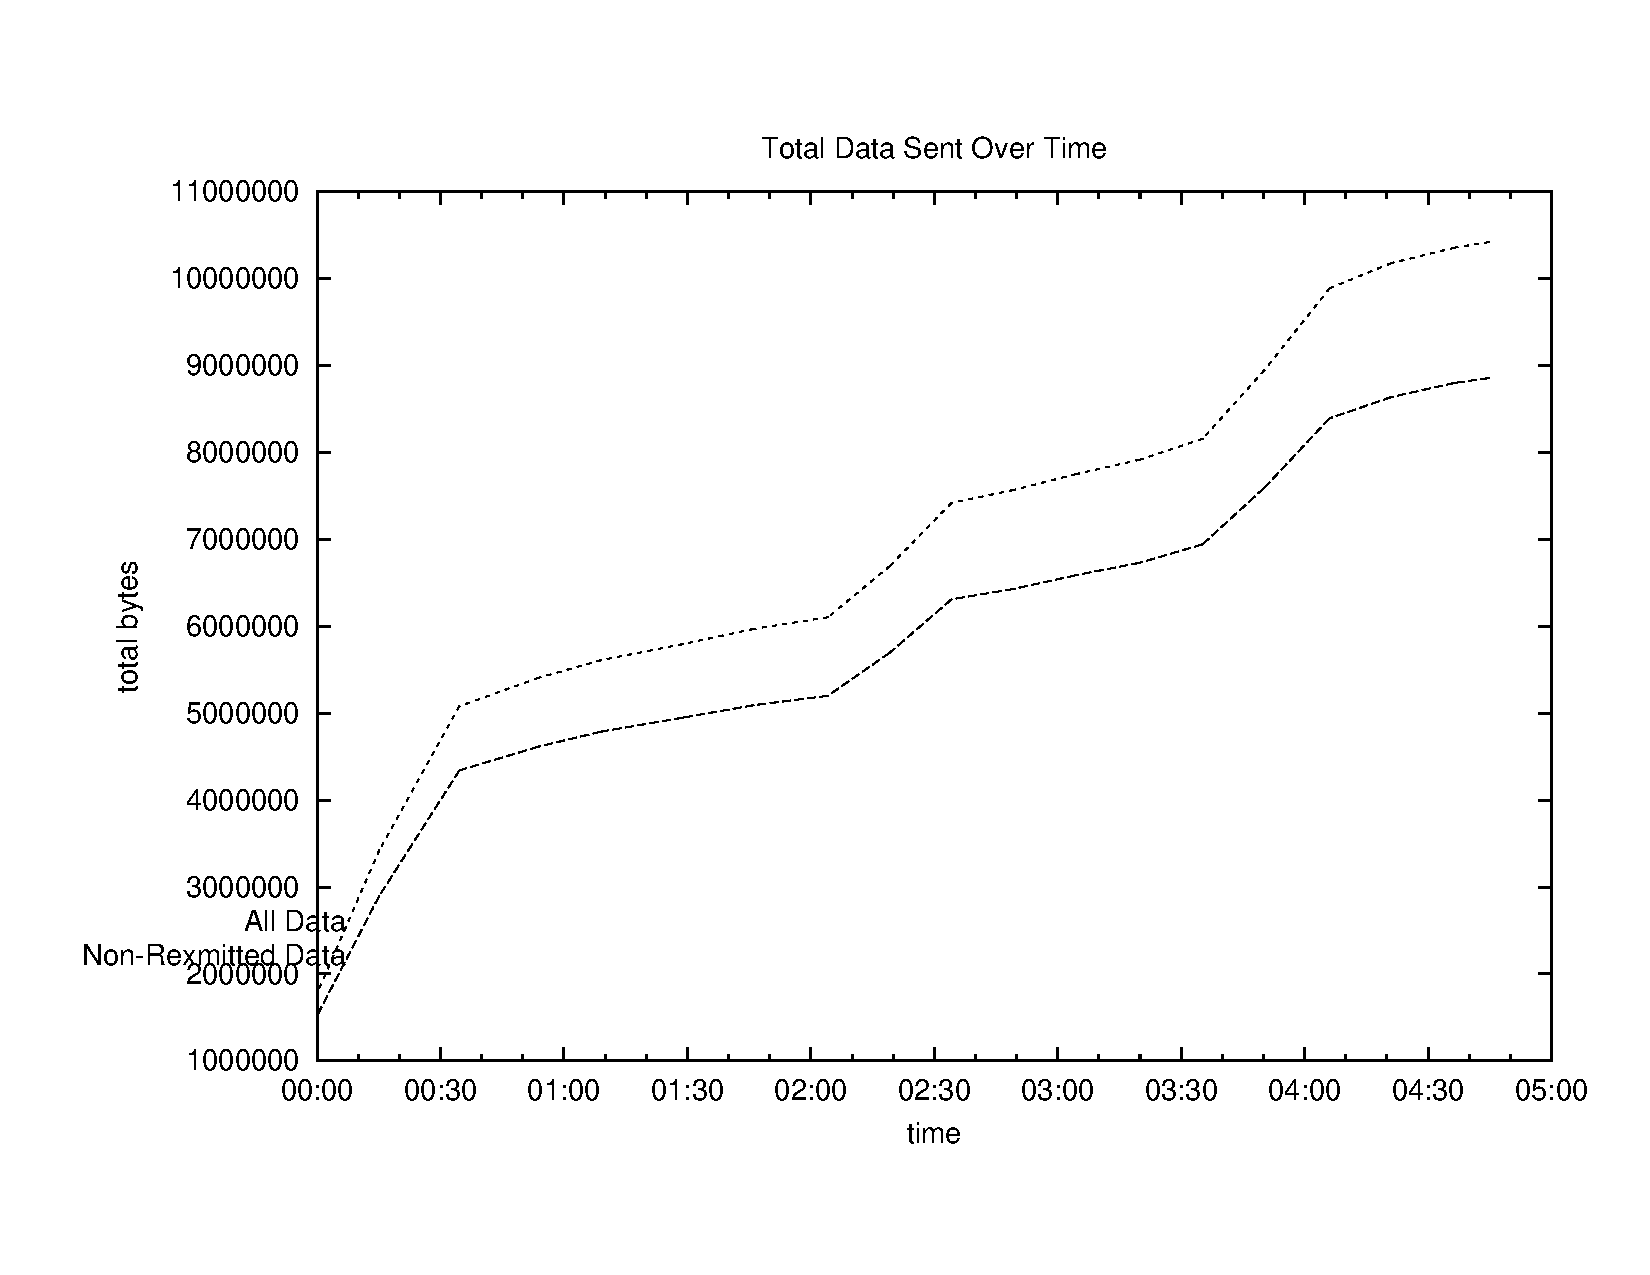
\includegraphics[height=10cm]{charts/dlna_traffic_15loss_data}
\caption{DLNA bad network traffic data chart \label{chart6}}
\end{figure}

\subsection{Statistics}
Through 16 months' releasing, our application have reached 924000 downloads from 223 countries all around the world, with around 10000 daily active users. This means our users almost cover 99% of the earth, a world map of our users is shown in Figure \ref{user_map}. So far, we got ratings from 10253 users, currently the average rating is 3.9 out of 5. The distribution is shown in Figure \ref{ratings}.

\begin{figure}[htb]
\centering 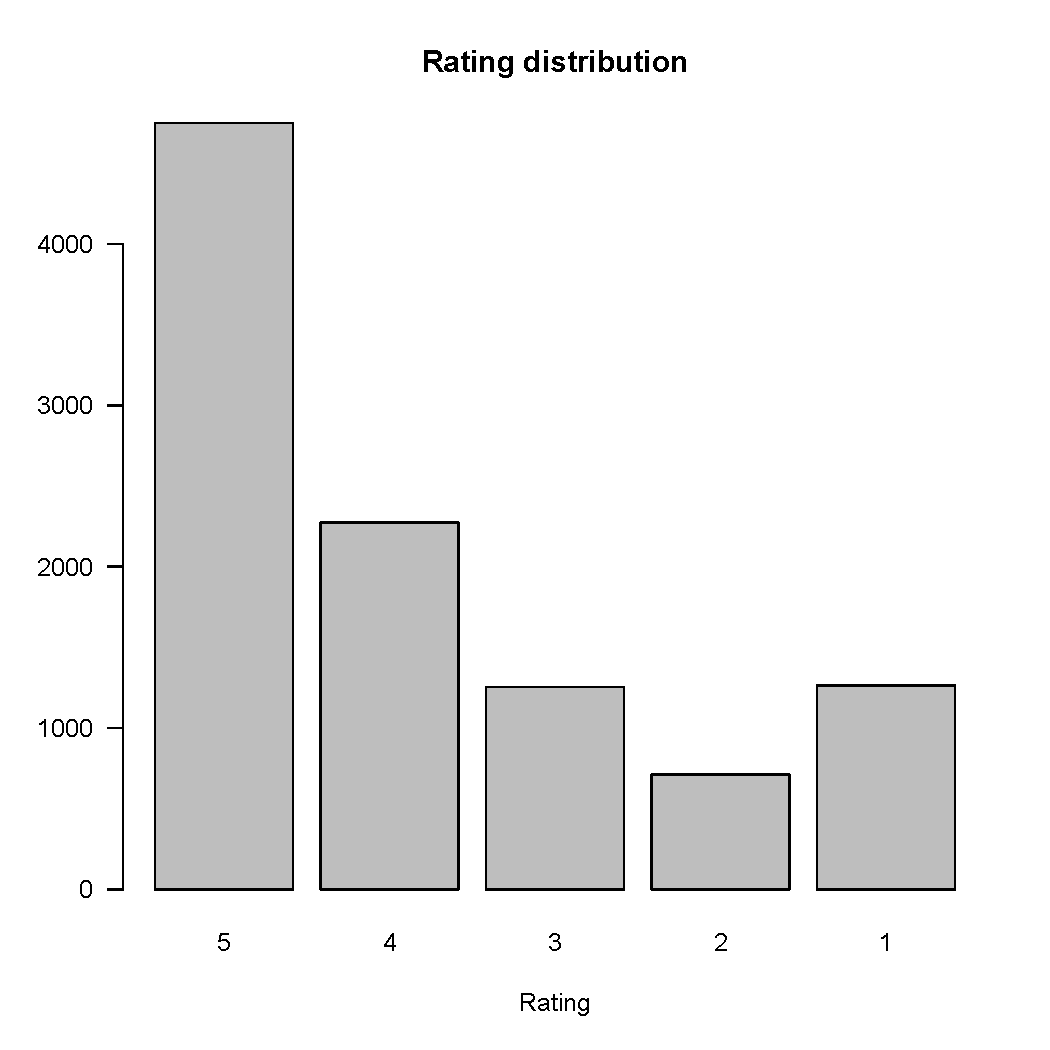
\includegraphics[height=9cm]{charts/rating_distribution}
\caption{Rating distribution\label{ratings}}
\end{figure}


The application turns out to be popular in countries like France, United States, Germany, United Kingdom and Brazil. The user distribution is shown in Figure \ref{user_country}.

\begin{figure}[htb]
\centering 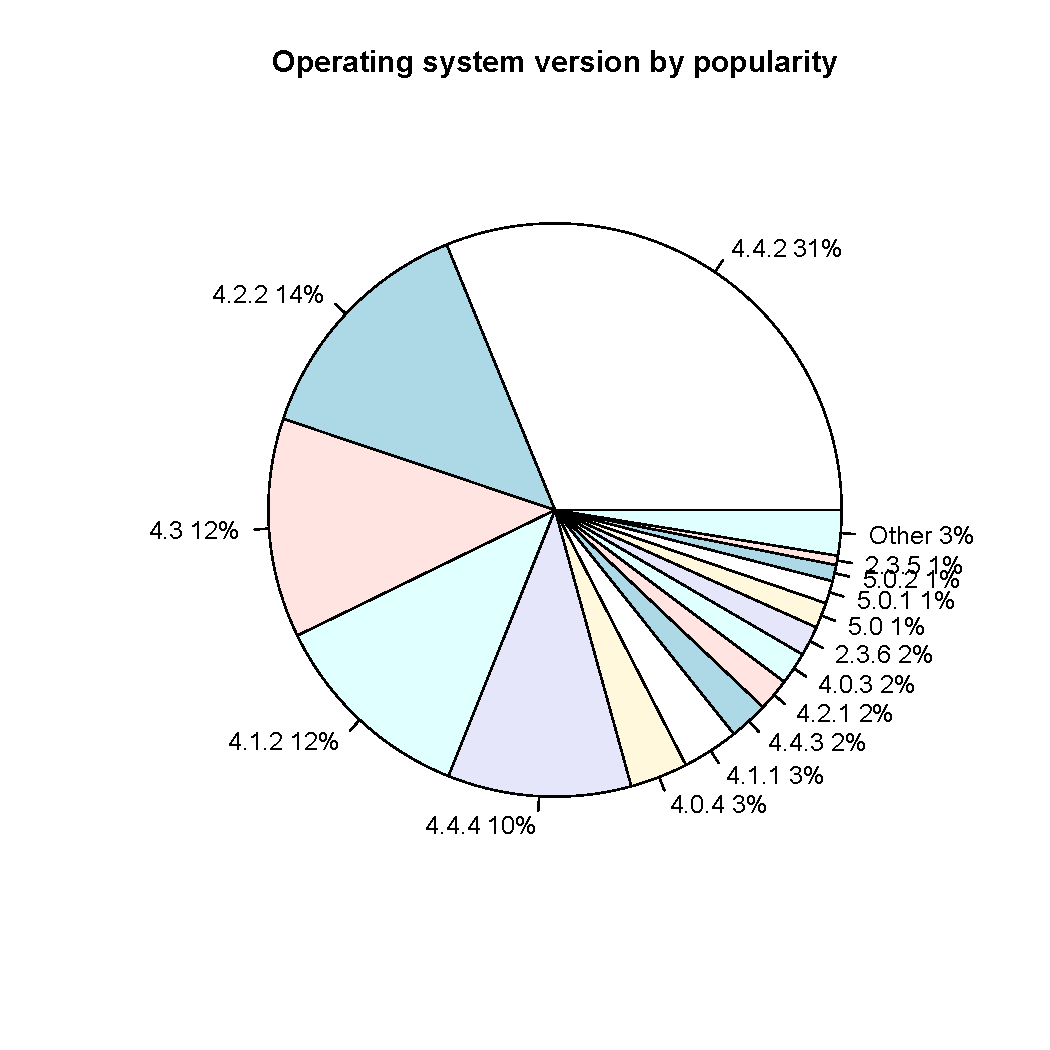
\includegraphics[height=9cm]{charts/os_version_popularity}
\caption{Popularity of different Android versions \label{os_versions}}
\end{figure}

\begin{figure}[htb]
\centering 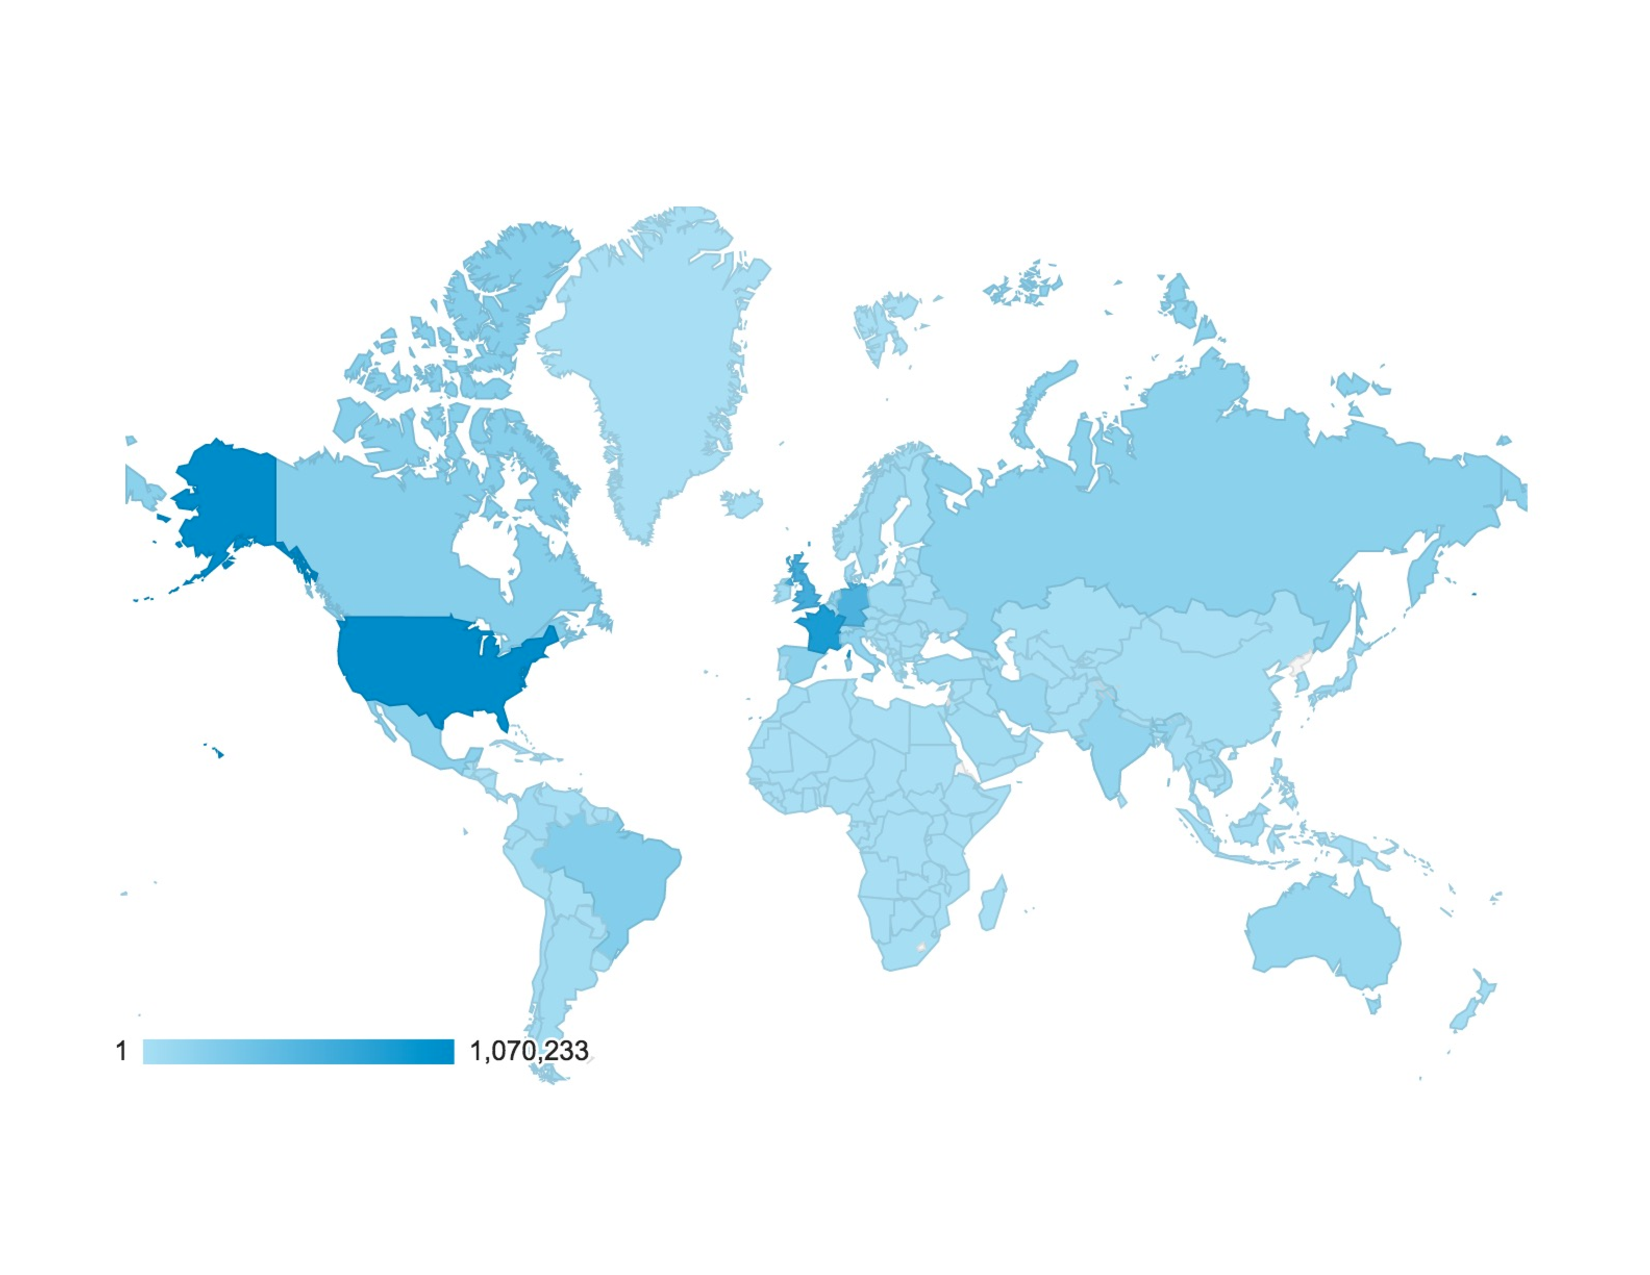
\includegraphics[width=9cm]{charts/session_world_map}
\caption{World map of visits \label{user_map}}
\end{figure}

\begin{figure}[htb]
\centering 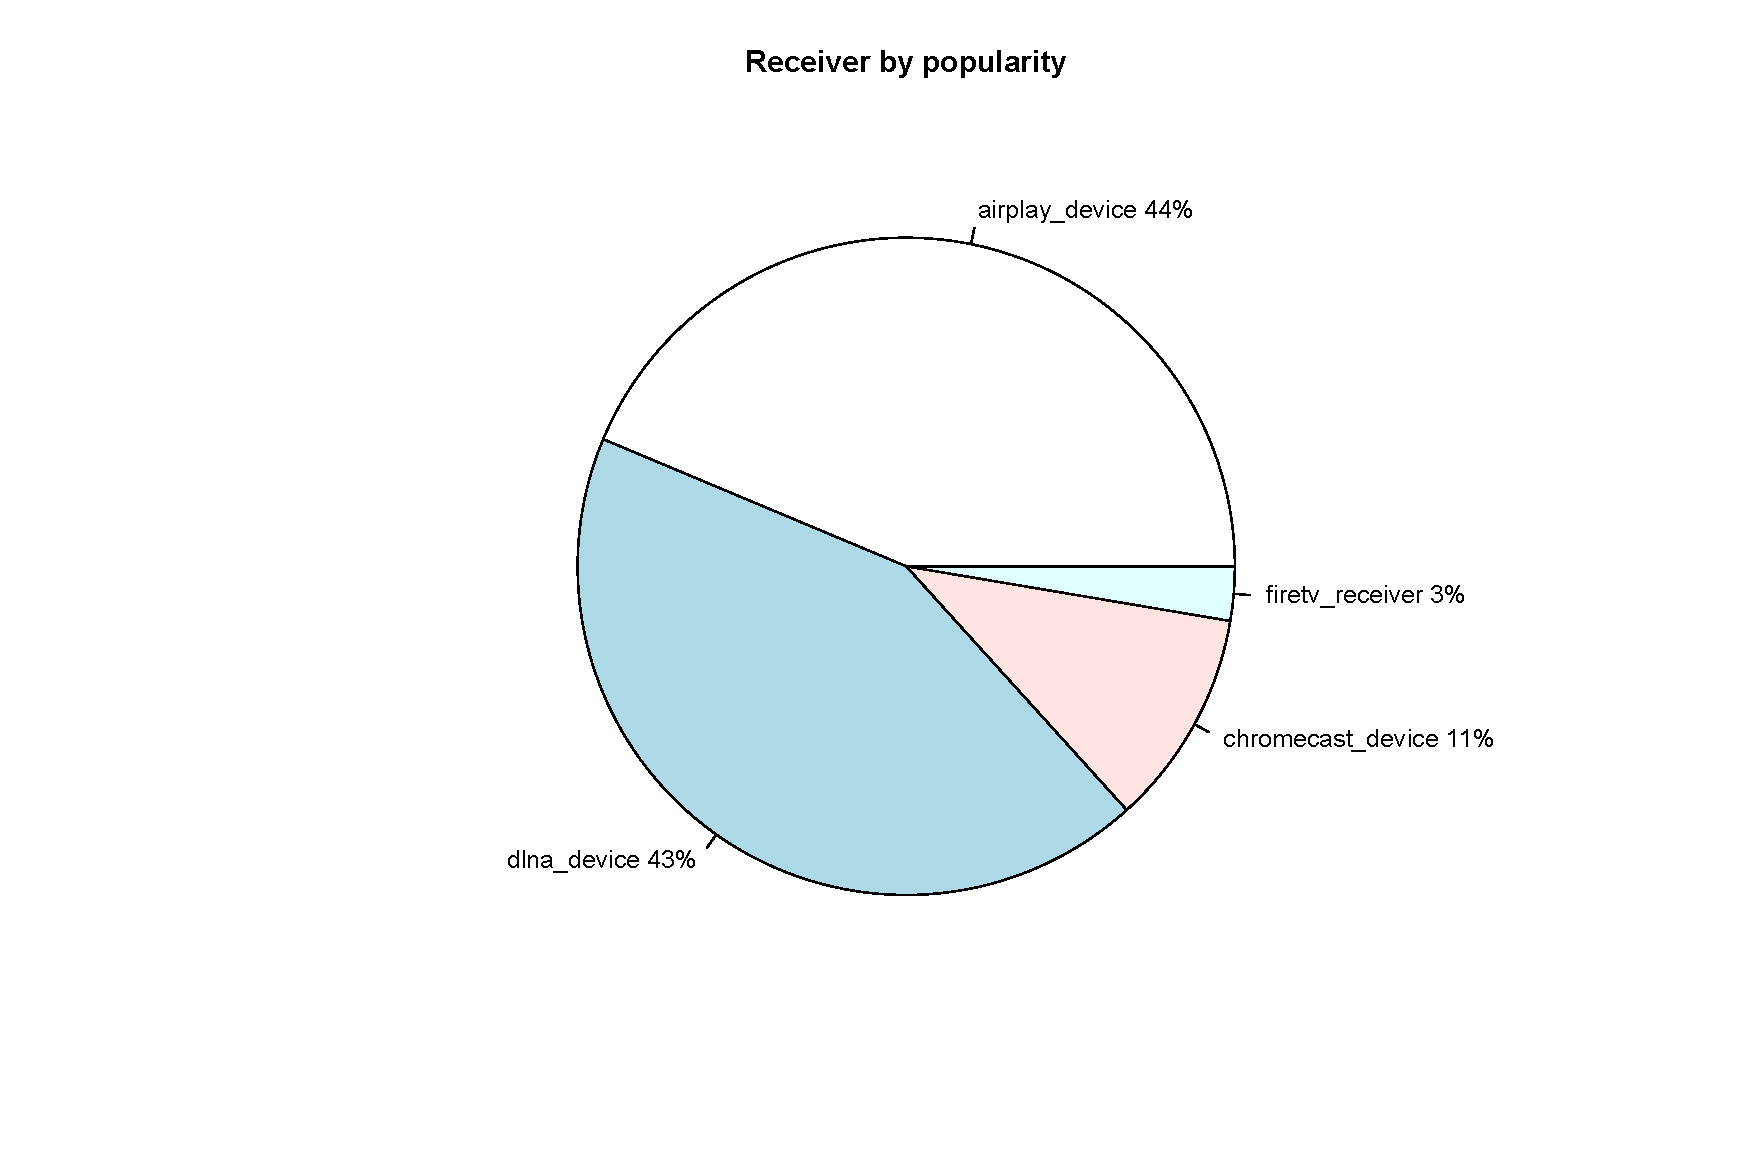
\includegraphics[height=9cm]{charts/receiver_popularity}
\caption{Popularity of receiver types \label{receiver_types}}
\end{figure}

\begin{figure}[htb]
\centering 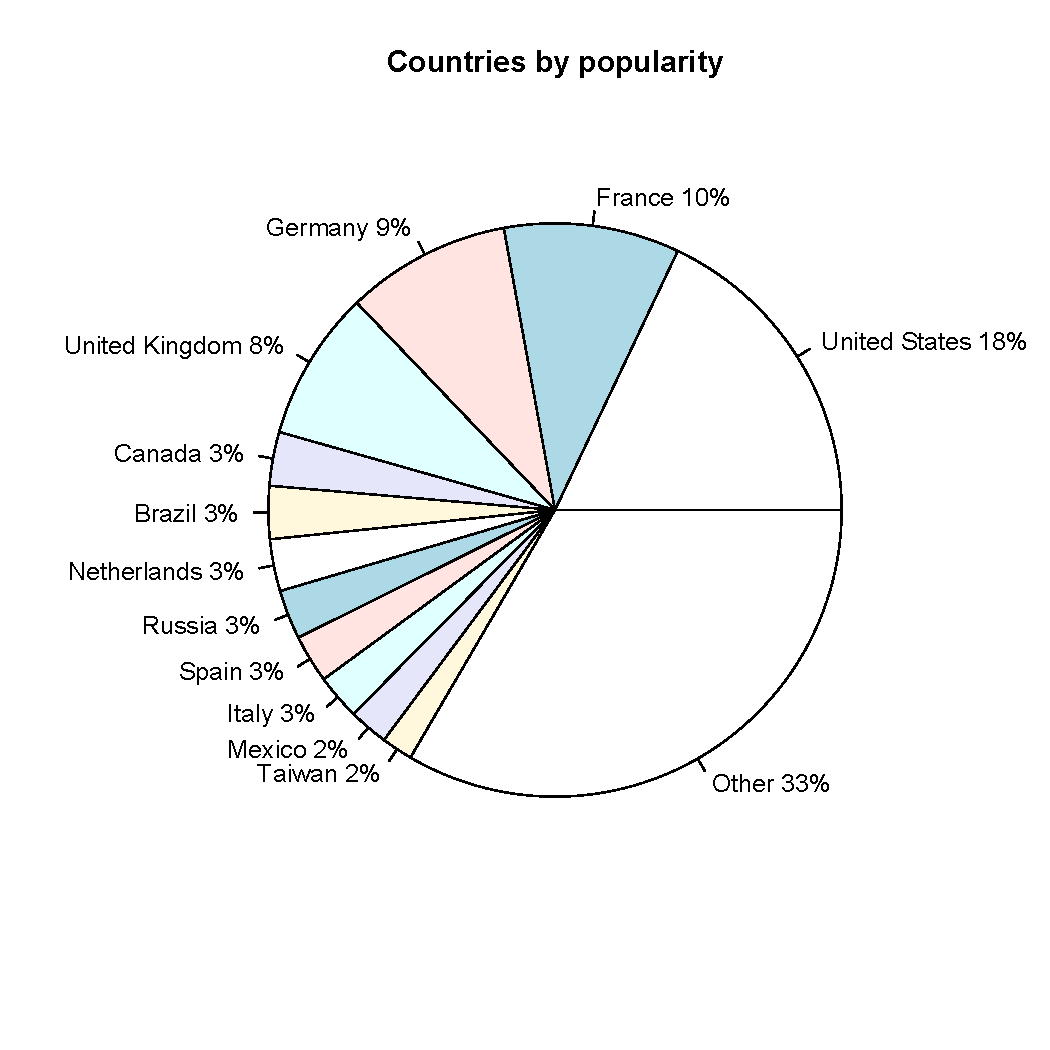
\includegraphics[height=9cm]{charts/country_popularity}
\caption{Popularity in different countries \label{user_country}}
\end{figure}


\begin{figure}[htb]
\centering 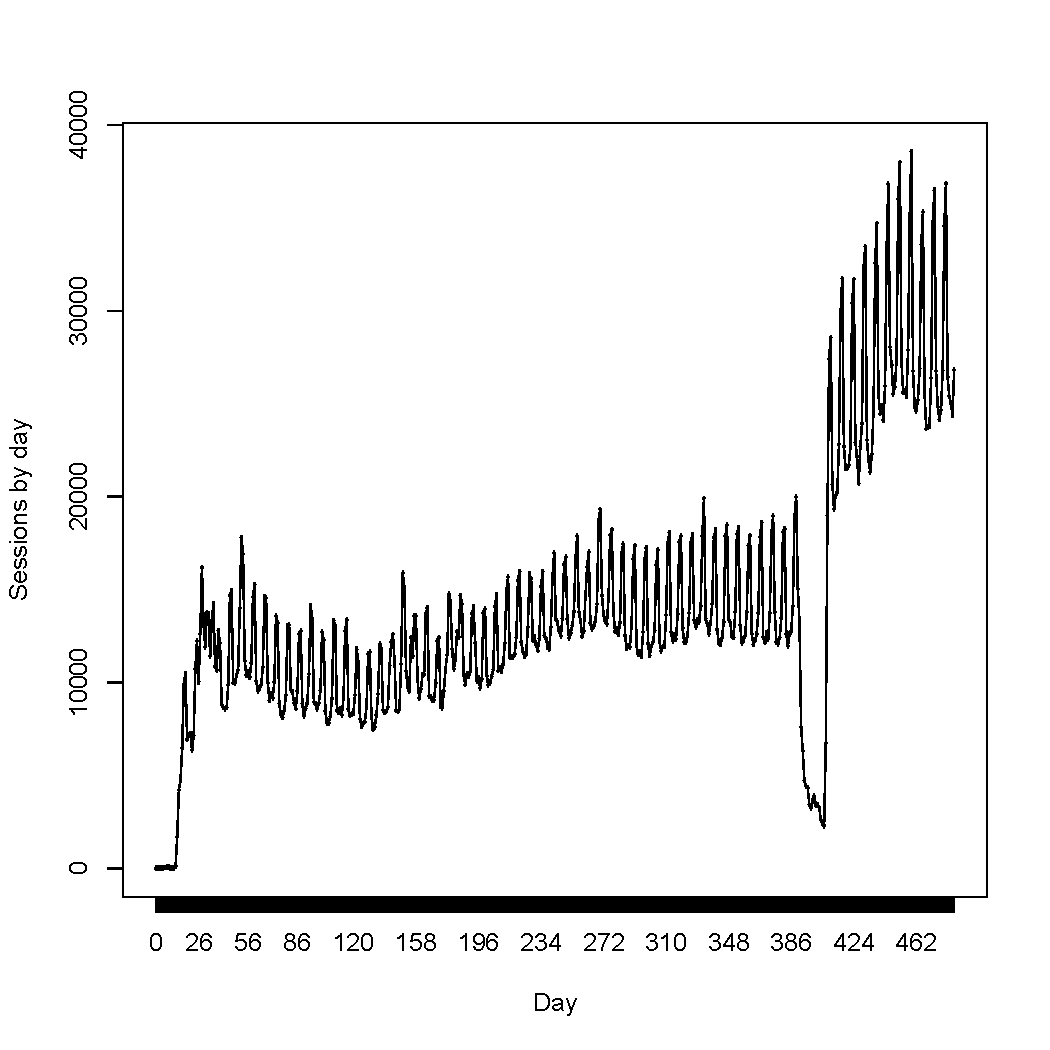
\includegraphics[height=9cm]{charts/sessions_per_day}
\caption{Sessions per day \label{sessions_perday}}
\end{figure}


\subsection{User study}
\begin{itemize}
\item[--]What information we can get back from users
\item[--]User behavior/ statistics
\item[--]Improve the application accordingly
\item[--]Strategies for decision making
\end{itemize}
Write result here.